\vbox to \myposterheight{%

%----------------------------------------------------------------------------------------
%	DECONVOLUTION
%----------------------------------------------------------------------------------------
\begin{block}{Deconvolution of ultrasound images}
	\begin{itemize}
		\item The proposed model relates the low-resolution RF image with the high-resolution TRF 
		\item It can be used for \textbf{deconvolution} \textit{i.e.} to retrieve the TRF from the DAS image 
		\item Let us define the RF image $\vect{s} \in \mathbb{R}^{N_{\Omega}}$ and the unknown TRF $\vect{\gamma} \in \mathbb{R}^{N_{\Omega}}$ over the spatial grid $\Omega = \left\lbrace \ser{\vect{r}}{j}, j = 1, \dots, N_{\Omega}\right\rbrace$
		\item The estimate of the TRF can be expressed from the RF image as:
		\begin{equation}
			\label{eq_deconv_pb}
			\vect{\gamma} \in \arg \min \limits_{\hat{\vect{\gamma}} \in \mathbb{R}^{N_{\Omega}}} \| \hat{\vect{\gamma}} \|_p \textnormal{ subject to } \| \mat{H} \hat{\vect{\gamma}} - \vect{s} \| \leq \epsilon
		\end{equation}
		where $p \in \left]0, 2\right]$ and $\mat{H} \in \mathbb{R}^{N_{\Omega} \times N_{\Omega}}$ is defined by:
		\begin{equation*}
			H_{jk} = PSF \left(\ser{\vect{r}}{j}, \ser{\vect{r}}{k}\right), \; \forall \left(\ser{\vect{r}}{j}, \ser{\vect{r}}{k}\right) \in \Omega^2 
		\end{equation*}
	\end{itemize}
\end{block}
\vfill

%----------------------------------------------------------------------------------------
%	EXPERIMENTAL SETTINGS
%----------------------------------------------------------------------------------------
\begin{block}{Experimental settings}
	\begin{itemize}
		\item Comparison with state-of-the-art deconvolution approaches which use spatially-invariant PSF~\cite{Chen2015}
		\item Raw-data simulated on Field II:
		\begin{itemize}
			\item 64-elements phased-array
			\item Central frequency $f_c$ = \SI{2.5}{\mega\hertz}, bandwidth of \SI{80}{\percent} 
			\item Sampling frequency $f_s$ = 
		\end{itemize}
		\item Standard DAS algorithm used to obtain the RF image
		\item Problem~\eqref{eq_deconv_pb} solved with Alternating direction method of multipliers~(ADMM)~\cite{Boyd2010} with $p=1$, $\epsilon = $ and \num{1500} iterations
	\end{itemize}
\end{block}
\vfill

%----------------------------------------------------------------------------------------
%	RESULTS
%----------------------------------------------------------------------------------------
\begin{block}{Results: Point-scatterers and foetus phantoms}
	\newlength{\PointFigWidth} \setlength{\PointFigWidth}{0.32\textwidth}
	\newlength{\PointFigHeight}
	\settoheight{\PointFigHeight}{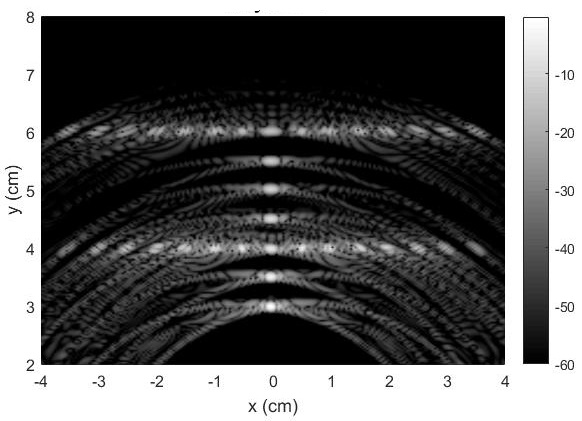
\includegraphics[width=\PointFigWidth]{figures/RF_image.jpg}}
	\newlength{\FoetusFigHeight}
	\settoheight{\FoetusFigHeight}{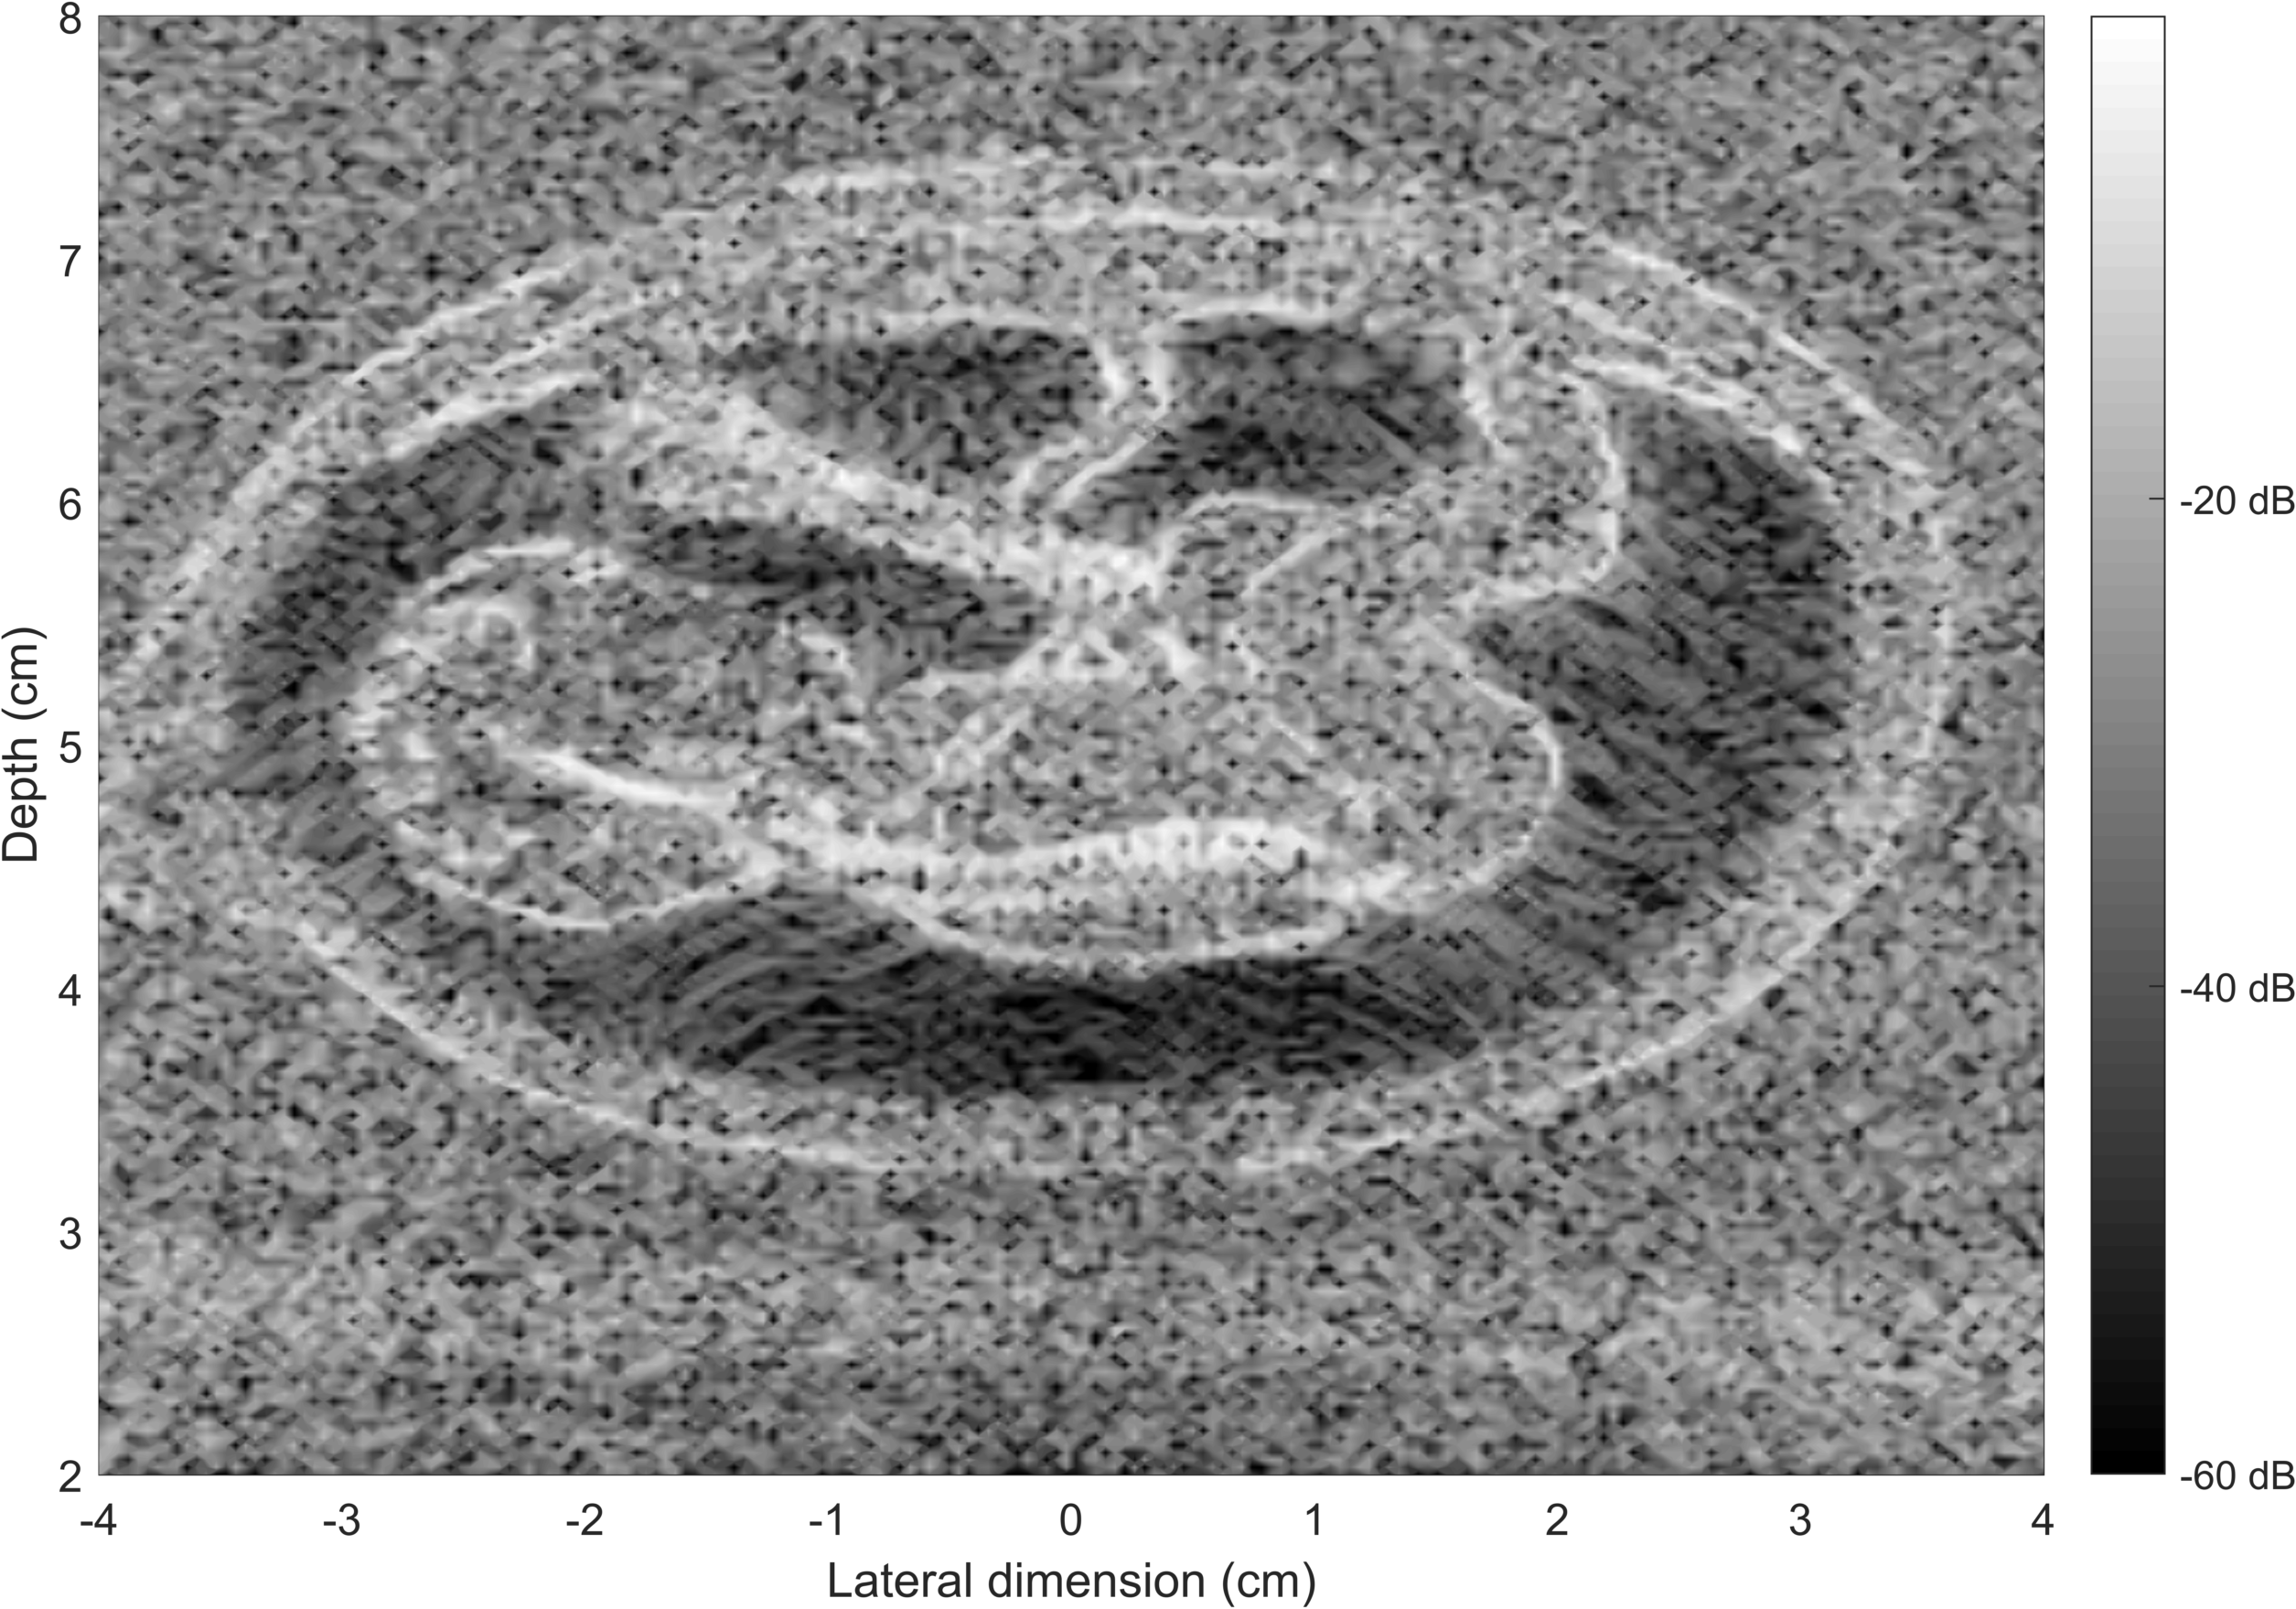
\includegraphics[width=\PointFigWidth]{figures/foetus_example.png}}
	\begin{figure}
		\centering
		% Maximum length
		\subcaptionbox{ }{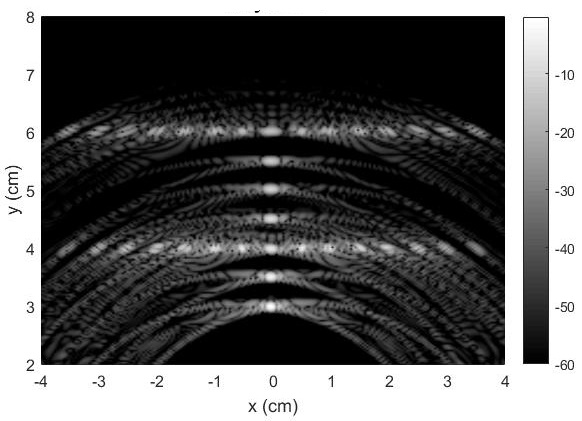
\includegraphics[height=\PointFigHeight]{figures/RF_image.jpg}}
		\subcaptionbox{ }{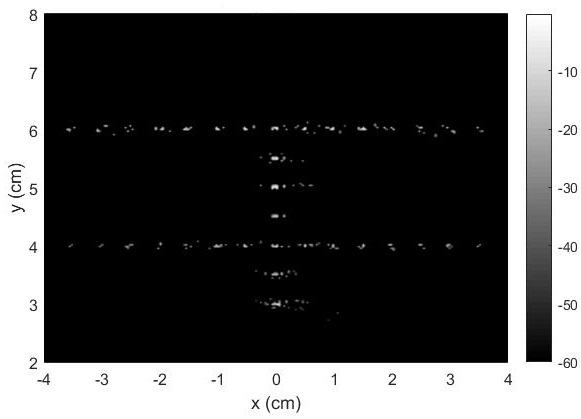
\includegraphics[height=\PointFigHeight]{figures/Deconv_varying_PSF.jpg}}
		\subcaptionbox{ }{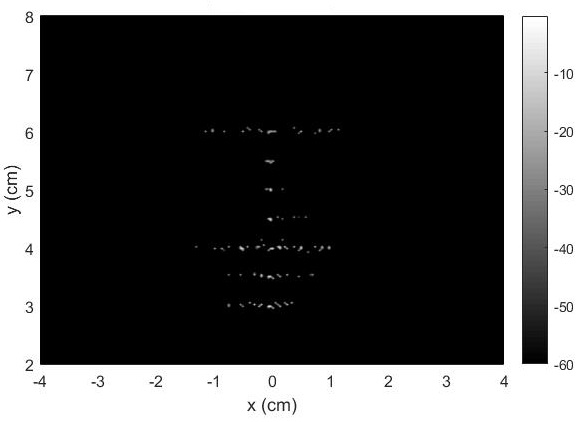
\includegraphics[height=\PointFigHeight]{figures/Deconv_cons_PSF.jpg}}
		~
		\subcaptionbox{ }{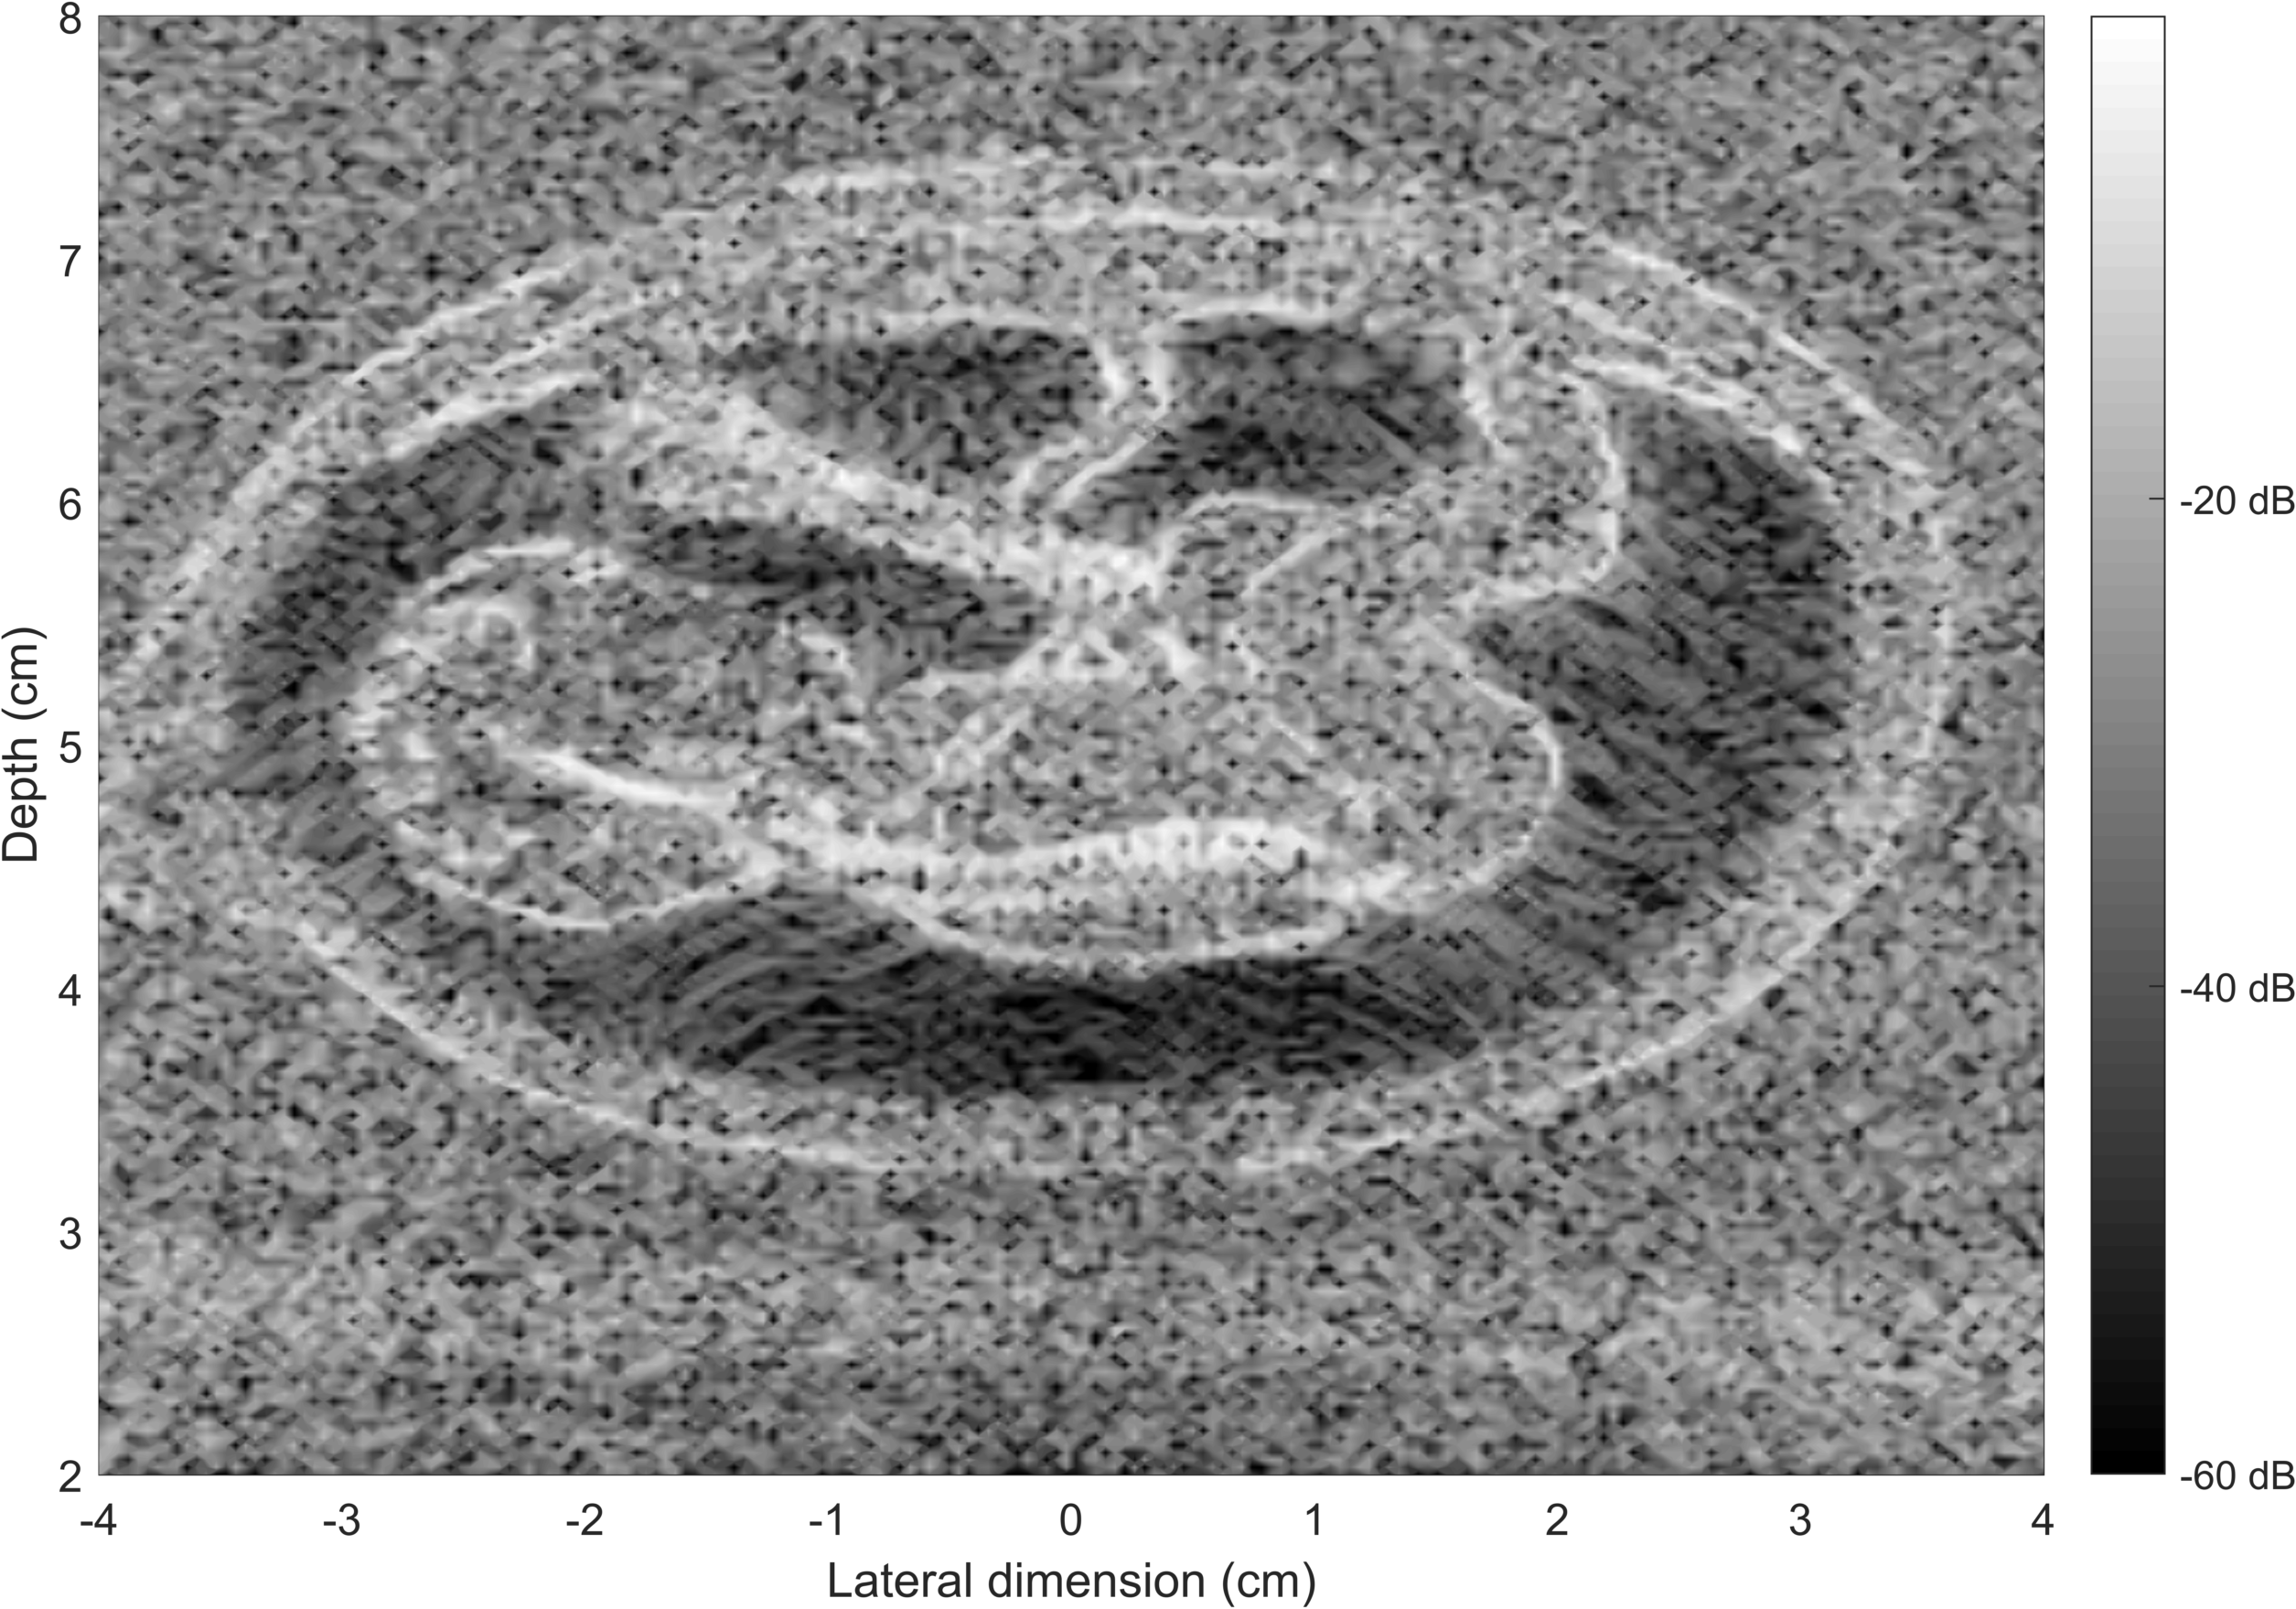
\includegraphics[height=\FoetusFigHeight]{figures/foetus_example.png}}
		\subcaptionbox{ }{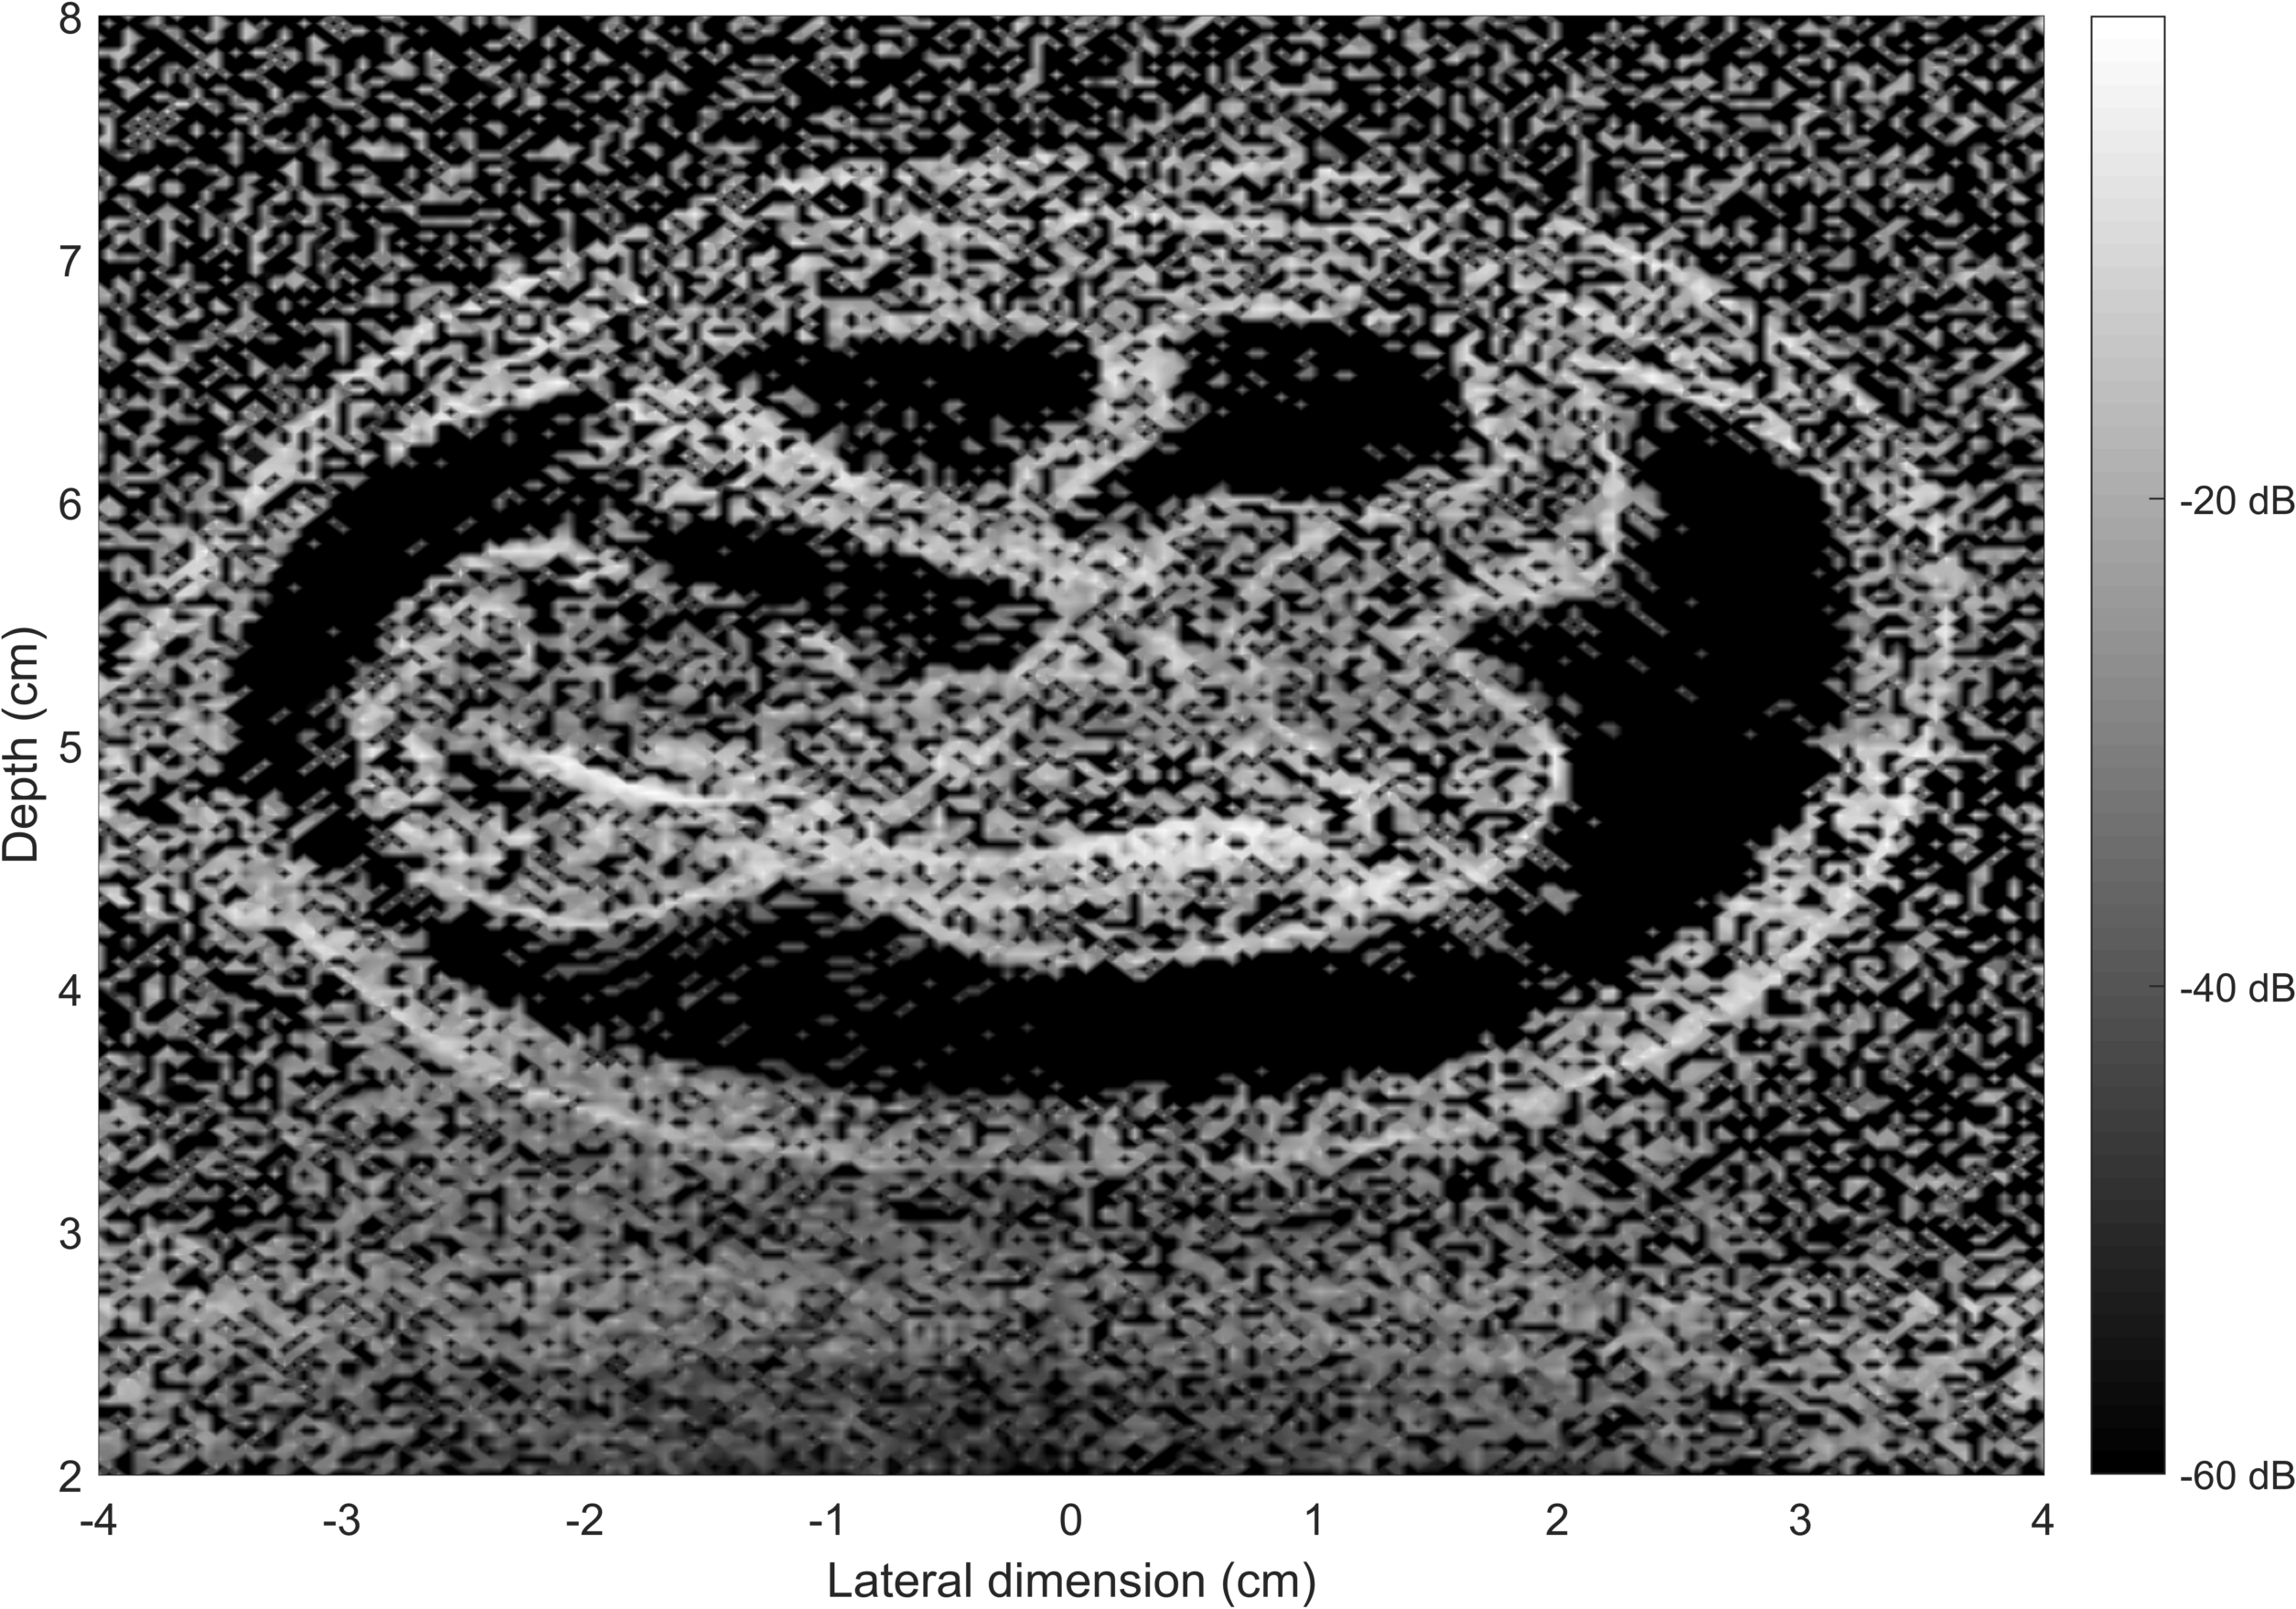
\includegraphics[height=\FoetusFigHeight]{figures/foetus_deconv_var.png}}
		\subcaptionbox{ }{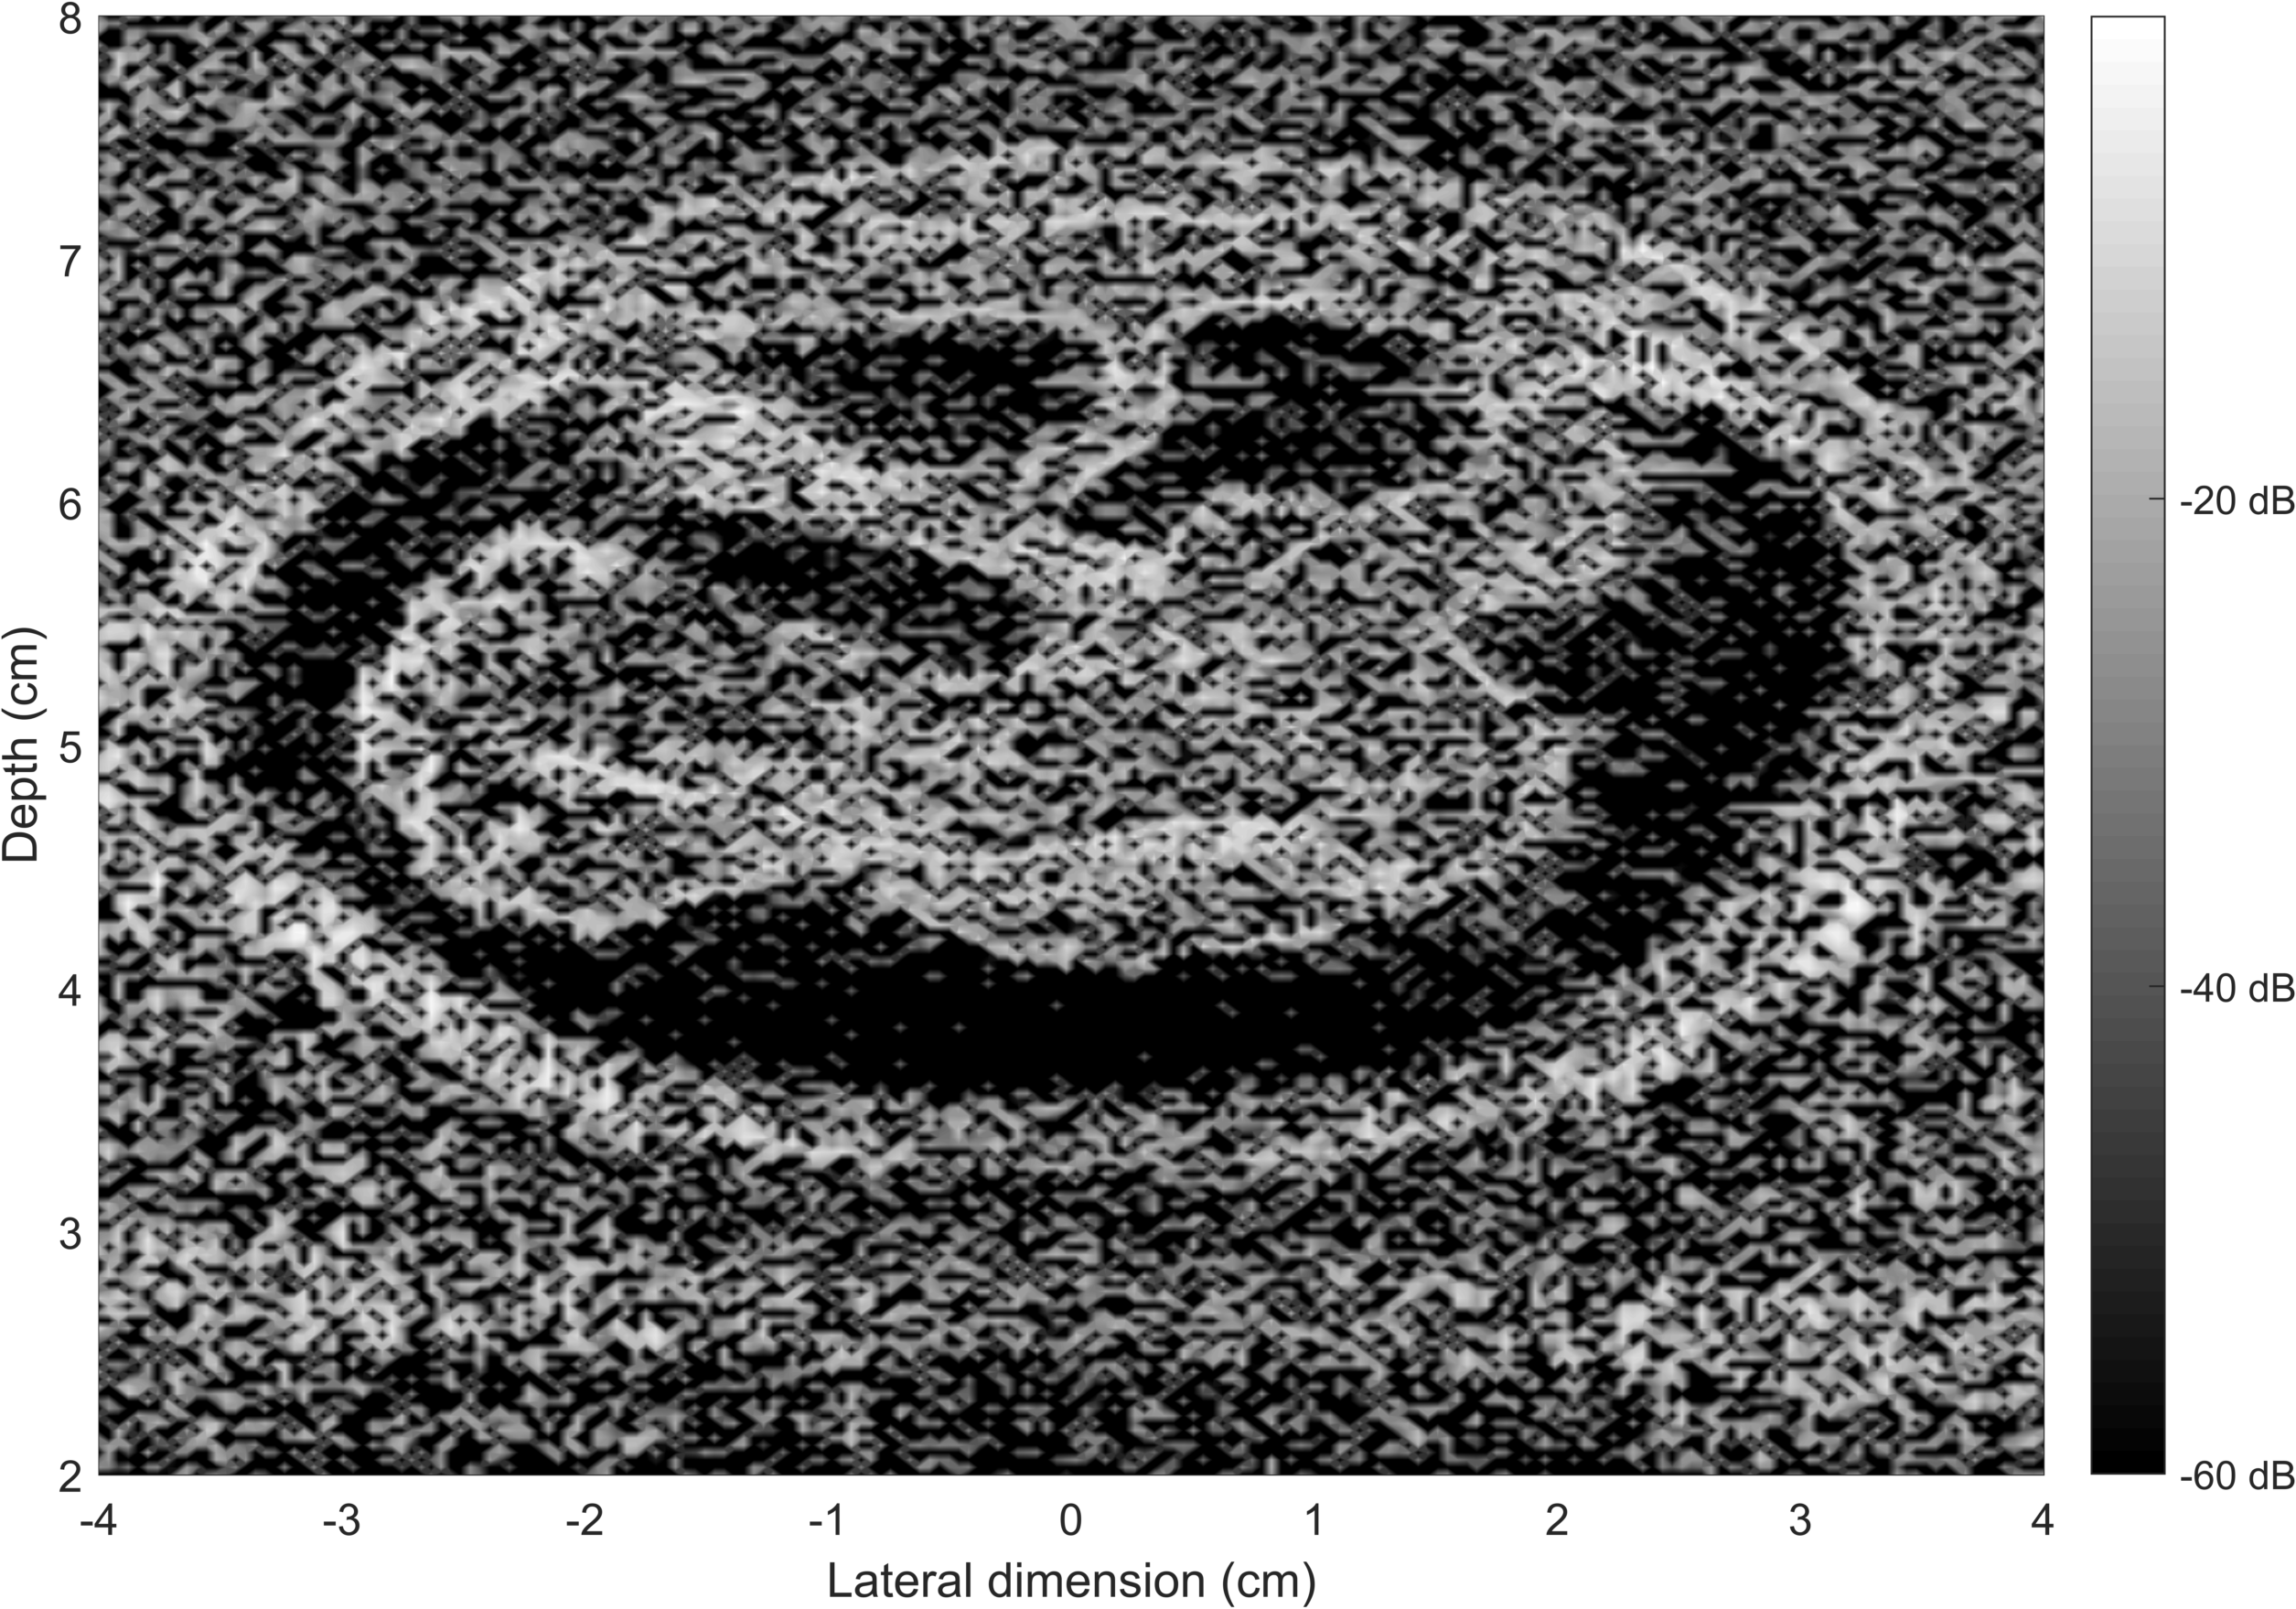
\includegraphics[height=\FoetusFigHeight]{figures/foetus_deconv_cst.png}}
		\caption{(a) RF image of the point-reflectors phantom; (b) Deconvolved image with the proposed operator; (c) Deconvolved image with spatially invariant PSF; (d) RF image of the foetus phantom; (e) Deconvolved image with the proposed operator; (f) Deconvolved image with spatially invariant PSF.}
	\end{figure}

\end{block}
\vfill

%----------------------------------------------------------------------------------------
%	CONCLUSION
%----------------------------------------------------------------------------------------

\begin{block}{Conclusion}
	
\end{block}
\vfill

%----------------------------------------------------------------------------------------
%	BIBLIOGRAPHY
%----------------------------------------------------------------------------------------

\begin{block}{References}
	\printbibliography
\end{block}
}